\documentclass{beamer}
\usepackage[utf8]{inputenc}   % pour pouvoir taper les accents directement     
\usepackage{amsfonts,amssymb,amsmath}
\usepackage{tikz}
\usepackage{array}
\usepackage{calc}
\usetikzlibrary{patterns}
\usepackage[absolute,showboxes,overlay]{textpos}     
\textblockorigin{0pt}{0pt}                          
\TPshowboxesfalse  
 \usepackage{lmodern,multido}

\newcommand{\R}{\mathbb{R}}
\newcommand{\C}{\mathbb{C}}
\newcommand{\Z}{\mathbb{Z}}
\newcommand{\N}{\mathbb{N}}
\newcommand{\Q}{\mathbb{Q}}
\newcommand{\E}{(-4,-1) rectangle (4,4)}
\newcommand{\A}{(0,0) ++(135:2) circle (2)}
\newcommand{\B}{(0,0) ++(45:2) circle (2)}

\begin{document}
 %%%%%%%%%%%%%%%%%%%%%%%%%%%%%%%%%%%%%%%%%%%%%%%%%%%%%%%%%%%%%%%

 \addtobeamertemplate{navigation symbols}{}{ \hspace{1em}    \usebeamerfont{footline}%
    \insertframenumber/\inserttotalframenumber }

 %%%%%%%%%%%%%%%%%%%%%%%%%%%%%%%%%%%%%%%%%%%%%%%%%%%%%%%%%%%%%%%

\begin{frame}{Introduction aux statistiques}
\begin{textblock*}{\textwidth}(1cm,2cm)

\begin{center}{\bf \Large Chapitre 1} \end{center}
\begin{center}{\bf \Large Variables aléatoires discrètes} \end{center}
\vspace{0.3cm}
\begin{itemize}
\item Définition d'une variable aléatoire 
\item Type de variables aléatoires
\item Caractéristiques d'une variable aléatoire discrète
\item Lois usuelles discrètes 
\begin{itemize}
\item Loi de Bernoulli
\item Loi Binomiale
\item Loi de Poisson
\item Approximations
\end{itemize}
\end{itemize}

 \end{textblock*}

\end{frame}

\section{Introduction}
\begin{frame}{Les variables aléatoires}

Si $\Omega $  = ensemble fondamental  associé à une expérience aléatoire :
\begin{itemize}
\item une population 
\item l'ensemble de tous les échantillons de taille $n$ d'une population donnée
\end{itemize}.
Une {\bf variable aléatoire} est une fonction $X:\Omega \longrightarrow \mathbb{R}$.

\

Exemple : $\Omega=\{ $adultes en Europe$\}$ et $X$ est :
\begin{itemize}
\item nombre d'enfants
\item taille
\item taux de glycémie...
\end{itemize} 
\end{frame}


%%%%%%%%%%%%%%%%%%%%%%%%%%%%%%%%%%%%%%%%%%%%%%%%%%%%%%%%%%%%%%%

\begin{frame}{Les variables aléatoires}

Deux types de variables aléatoires :
 \begin{itemize}
\item {\bf discrète} si ensemble des 
valeurs =  ensemble fini ou infini dénombrable (comme $\mathbb{\N}$).
\item  {\bf continue} si ensemble des valeurs = intervalle de $\mathbb{R}$.
\end{itemize}

\

On caractérise une variable aléatoire par :
 \begin{itemize}
\item une distribution ou loi de probabilité : à chaque valeur est associée une probabilité \\
Densité de probabilité ou fonction de répartition 
\item une tendance centrale : l'espérance mathématique 
\item la dipersion des valeurs : la variance ou l'écart-type
\end{itemize}

\end{frame}

%%%%%%%%%%%%%%%%%%%%%%%%%%%%%%%%%%%%%%%%%%%%%

\begin{frame}{Les variables aléatoires}
\begin{textblock*}{\textwidth}(1cm,2cm)
La {\bf fonction de répartition} d'une variable aléatoire $X$ est  
$$F:\mathbb{R}\longrightarrow [0\,;\,1]\mbox{ définie par
 }
F(x)=Pr(X\leq x)\,.
$$
\end{textblock*}


\begin{textblock*}{\textwidth}(1cm,5cm)

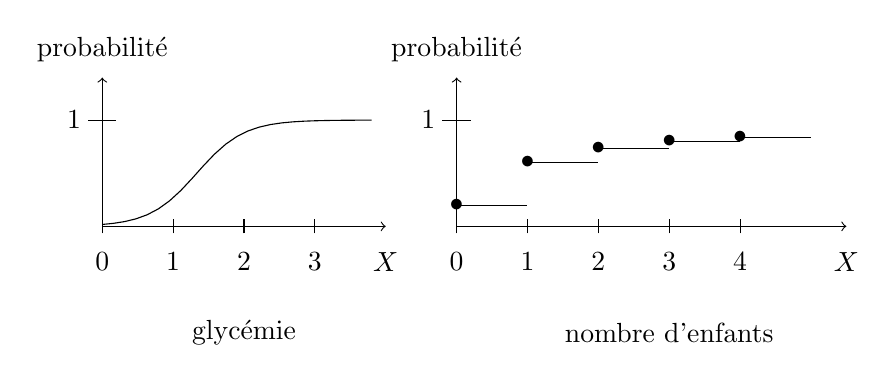
\begin{tikzpicture}[scale=0.9]
\draw [domain=0:3.8] plot (\x,{1.5+1.5*exp(2*(1.5*\x-2))/(exp(2*(1.5*\x-2))+1});
\draw[->](0,1.5)--(0,3.6);
\draw[->](0,1.5)--(4,1.5);
\multido{\i=0+1}{4}{%
\draw (\i,1.4) -- (\i,1.6);
\draw (\i,1) node {\i};}
\draw (2,0) node {glycémie} ;
\draw (4,1) node {$X$} ;
\draw (0,4) node {probabilité} ;
\draw (-0.2,3) -- (0.2,3);
\draw (-0.4,3) node {1};
\draw[->](5,1.5)--(5,3.6);
\draw[->](5,1.5)--(10.5,1.5);
\multido{\i=0+1}{5}{%
\draw (\i+5,1.4) -- (\i+5,1.6);
\draw (\i+5,1) node {\i};
}
\multido{\i=1+1}{5}{%
\draw (\i+4,3-1.2/\i) -- (\i+5,3-1.2/\i) ;
\draw (\i+4,3-1.2/\i) node {$\bullet$};
}
\draw (8,0) node {nombre d'enfants} ;
\draw (10.5,1) node {$X$} ;
\draw (5,4) node {probabilité} ;
\draw (4.8,3) -- (5.2,3);
\draw (4.6,3) node {1};
\end{tikzpicture}

\end{textblock*}

\end{frame}

%%%%%%%%%%%%%%%%%%%%%%%%%%%%%%%%%%%%%%%%%%%%%



\begin{frame}{Les variables aléatoires}
\begin{textblock*}{\textwidth}(1cm,2cm)
La {\bf fonction de répartition} d'une variable aléatoire $X$ 
$$F:\mathbb{R}\longrightarrow [0\,;\,1]\mbox{ définie par
 }
F(x)=Pr(X\leq x)\,.
$$
\end{textblock*}

\begin{textblock*}{\textwidth}(1cm,5cm)

Propriétés :
\begin{itemize}
\item $Pr(a<X\leq b)=F(b)-F(a)$
\item $F$ est croissante et continue \`a droite
\item $\displaystyle \lim\limits_{-\infty} F(x)=0$ et $\displaystyle \lim\limits_{+\infty} F(x)=1$
\item $Pr(X>a)=1-Pr(X\leq a)$\\
\end{itemize}
\end{textblock*}

\end{frame}




%%%%%%%%%%%%%%%%%%%%%%%%%%%%%%%%%%%%%%%%%%%%%

\begin{frame}{Les variables aléatoires discrètes}
%{\Large Variable discrète :}

\only<1>{
\begin{itemize}

\item  $X(\Omega)=\{x_1,\hdots, x_n \}$  :
 loi de $X$  entièrement déterminée par
 $$Pr(X=x_1), \hdots, Pr(X=x_n)$$ avec  $\sum\limits_{k=1}^n Pr(X=x_k) =1$.
 
{\bf Espérance}  de $X$ :
$
E(X)=\sum\limits_{k=1}^n x_k Pr(X=x_k).
$
\end{itemize}
}

\only<2>{
\begin{itemize}
\item   $X(\Omega)=\mathbb{\N}$ :  loi de $X$ est entièrement déterminée
par $$Pr(X=k), \ k \in \mathbb{\N}$$ avec $\sum\limits_{k=0}^\infty Pr(X=k) =1$.

{\bf Espérance}  de $X$ :
$
E(X)=\sum\limits_{k=1}^\infty k Pr(X=k).
$
\end{itemize}
}

\

{\bf Variance :} $Var(X)=E(X^2)-E(X)^2$ 

{\bf Écart-type :} $\sigma(X)=\sqrt{Var(X)}$.

\end{frame}


%%%%%%%%%%%%%%%%%%%%%%%%%%%%%%%%%%%%%%%%%%%%%

\begin{frame}{Les variables aléatoires  discrètes}

\noindent {\bf Variables aléatoires indépendantes :}\\

\

 $X$ et $Y$ discrètes à valeurs  dans $\{1,\ldots,I\}$
(resp . $\{1,\ldots,J\}$) sont indépendantes ssi 

\

$\forall i \in \{1,\ldots,I\} , \forall j \in \{1,\ldots,J\}$

$$Pr(X=i\;{\mbox { et }}\; Y=j)=Pr(X=i)\times Pr(Y=j).$$


\end{frame}

%%%%%%%%%%%%%%%%%%%%%%%%%%%%%%%%%%%%%%%%%%%%%

\begin{frame}{Les variables aléatoires discrètes}

\noindent {\large \bf Combinaison linéaire de variables aléatoires (discrètes ou continues) :} \\

\

$X$ et $Y$ deux variables aléatoires ;
$\alpha$ et $\beta$ deux réels.
\begin{itemize}
\item $E(\alpha X+\beta Y) =  \alpha E(X) + \beta E(Y)$.
\item si $X$ et $Y$ indépendantes, $Var(\alpha X+\beta Y) = \alpha^2 Var(X) + \beta^2 Var(Y)$ 
\end{itemize}

\

En particulier,  
$E(\alpha+ X) =  \alpha +E(X) $ et $Var(\alpha + X) =  Var(X) $ 

\end{frame}

 %%%%%%%%%%%%%%%%%%%%%%%%%%%%%%%%%%%%%%%%%%%%%%%%%%%%%%%%%%%%%%%

\begin{frame}{Lois usuelles discrètes}

\begin{center}{\bf \Large Loi de Bernoulli $B(p)$ avec $p\in[0;1]$} \end{center}
\begin{itemize}
\item  modélise une expérience de type pile ou face :
 la variable aléatoire $X$ ne prend que deux valeurs possibles (0 et 1)
 \item  paramètre $p$ : probabilité de succès (1)
 \item  la loi de $X$ est
$$
Pr(X=1)=p\quad {\mbox { et }} \quad Pr(X=0)=1-p\,.
$$


\end{itemize}
$E(X)=p$ et $Var(X)=p(1-p)$.


\end{frame}

 %%%%%%%%%%%%%%%%%%%%%%%%%%%%%%%%%%%%%%%%%%%%%%%%%%%%%%%%%%%%%%%

\begin{frame}{Lois usuelles discrètes}

\begin{textblock*}{\textwidth}(1cm,2cm)
\begin{center}{\bf \Large Loi Binomiale $\mathcal{B}(n\,;\,p)$ avec $n\in\mathbb{N}$ et $p\in[0;1]$} \end{center}
\begin{itemize}
\item  modélise le nombre de succès  dans $n$  répétitions  \textcolor{red}{indépendantes} d'un même schéma de Bernoulli $B(p)$
 \item  valeurs de $X$ : $\{0,1,2,\hdots,n\}$ 
 \item   loi de $X$ :
$$
Pr(X=k)=\begin{pmatrix}n\\k\end{pmatrix} p^k (1-p)^{n-k}\quad {\mbox { o\`u }} \begin{pmatrix}n\\k\end{pmatrix}= C_n^k=\frac{n!}{k!(n-k)!}\,.
$$
\end{itemize}

\noindent Rappel : $n\,!=n(n-1)(n-2)\hdots 1$ avec $0\, !=1$.



\end{textblock*}

\end{frame}

 %%%%%%%%%%%%%%%%%%%%%%%%%%%%%%%%%%%%%%%%%%%%%%%%%%%%%%%%%%%%%%%

\begin{frame}{Lois usuelles discrètes}

\begin{textblock*}{\textwidth}(1cm,2cm)
\begin{center}{\bf \Large Loi Binomiale $\mathcal{B}(n\,;\,p)$ avec $n\in\mathbb{N}$ et $p\in[0;1]$} \end{center}

\
 
 \

\noindent $E(X)=np$ et $Var(X)=np(1-p)$

\
 
 \



Si  $p$ probabilité qu'un individu possède une propriété, et $X$ variable  égale au nombre d'individus possédant cette propriété dans  échantillon de taille $n$ alors $X$ suit une loi binomiale $\mathcal{B}(n\,;\,p)$

(si variables aléatoires des $n$ Bernouillis indépendantes)

 
 




\end{textblock*}

\end{frame}

%%%%%%%%%%%%%%%%%%%%%%%%%%%%%%%%%%%%%%%%%%%%%








%%%%%%%%%%%%%%%%%%%%%%%%%%%%%%%%%%%%%%%%%%%%%

\begin{frame}{Lois usuelles discrètes}
\begin{textblock*}{\textwidth}(1cm,2cm)
\begin{center}{\bf \Large Loi de Poisson $\mathcal{P}(\lambda)$ avec $\lambda>0$ }\end{center}

\begin{itemize}
 \item ensemble des valeurs de $X$ : $\mathbb{N}$ 
 \item   loi de $X$ :
$$
Pr(X=k)=\frac{\lambda^k}{k !} e^{-\lambda} \,, \quad \forall k\in\mathbb{N}.
$$
\end{itemize}

 
\noindent On a $E(X)=Var(X)=\lambda$.\\

\

\


Loi des évènements rares
 \end{textblock*}
\end{frame}





%%%%%%%%%%%%%%%%%%%%%%%%%%%%%%%%%%%%%%%%%%%%%

\begin{frame}{Lois usuelles discrètes}
\begin{textblock*}{\textwidth}(1cm,2cm)
\begin{center}{Loi de Poisson $\mathcal{P}(\lambda)$ avec $\lambda>0$ }\end{center}

{\bf Stabilité par somme indépendante :}

\begin{itemize}
\item $X\sim \mathcal{P}(\lambda)$
\item $Y\sim \mathcal{P}(\mu)$ 
\item $X$ et $Y$ {\bf indépendantes}
\end{itemize}

alors  $X+Y\sim\mathcal{P}(\lambda+\mu)$.

 \end{textblock*}
\end{frame}


%%%%%%%%%%%%%%%%%%%%%%%%%%%%%%%%%%%%%%%%%%%%%%%%%%%%%%%%%%%%%%%

\begin{frame}{Approximations}
\begin{textblock*}{\textwidth}(1cm,2cm)
\begin{center}{\bf \Large Loi Binomiale et loi de Poisson } \end{center}

\begin{minipage}{0.4\textwidth}
Si 
\begin{itemize}
\item $X\sim \mathcal{B}(n,p)$ ;
\item $n$ grand : $n\geq 30$ ;
\item $p$ petit : $p\leq 0,1$ ;
\item $np$ "raisonnable" : $np\leq 10$ ;
\end{itemize}
\end{minipage}
\begin{minipage}{0.45 \textwidth}
\begin{center}
\begin{tikzpicture}[xscale=0.2,yscale=3.8]
\draw[->] (-0.5,0) -- (23,0);
\draw[->] (0,-0.01) -- (0,0.9);
%\foreach \n in {1,15}
%{
\only<1>
{
	\foreach \k in {0,...,20}
	{	
		\draw plot file {data/approx_binom_1_\k.txt} node {$\bullet$} ;
		\draw[red] plot file {data/approx_binom_poiss_1_\k.txt} node {$\times$} ;
	}	
\draw (20,0.7) node {$n=1$};
}
%}
\only<2>
{
	\foreach \k in {0,...,20}
	{	
		\draw plot file {data/approx_binom_8_\k.txt} node {$\bullet$} ;
		\draw[red] plot file {data/approx_binom_poiss_8_\k.txt} node {$\times$} ;
	}	
\draw (20,0.7) node {$n=8$};
}


\only<3>
{
	\foreach \k in {0,...,20}
	{	
		\draw plot file {data/approx_binom_15_\k.txt} node {$\bullet$} ;
		\draw[red] plot file {data/approx_binom_poiss_15_\k.txt} node {$\times$} ;
	}	
\draw (20,0.7) node {$n=15$};
}
%}

\end{tikzpicture}
\end{center}
\end{minipage}

alors $X$ suit approximativement une loi de Poisson $\mathcal{P}(np)$.
 

\end{textblock*}

\end{frame} 

%%%%%%%%%%%%%%%%%%%%%%%%%%%%%%%%%%%%%%%%%%%%%

\end{document}



%%%%%%%%%%%%%%%%%%%%%%%%%%%%%%%%%%%%%%%%%%%%%
\begin{frame}{Lois usuelles discrètes}

\begin{textblock*}{\textwidth}(1cm,2cm)
\begin{center}{\bf \Large Loi Binomiale $\mathcal{B}(n\,;\,p)$ avec $n\in\mathbb{N}$ et $p\in[0;1]$} \end{center}

\begin{center}
\only<1>{$n=1$ et $p=0.5$}
\only<2>{$n=2$ et $p=0.5$}
\only<3>{$n=3$ et $p=0.5$}
\only<4>{$n=4$ et $p=0.5$}
\only<5>{$n=5$ et $p=0.5$}
\only<6>{$n=6$ et $p=0.5$}
\only<7>{$n=7$ et $p=0.5$}
\only<8>{$n=8$ et $p=0.5$}
\only<9>{$n=9$ et $p=0.5$}
\only<10>{$n=10$ et $p=0.5$}
\only<11>{$n=11$ et $p=0.5$}
\only<12>{$n=12$ et $p=0.5$}
\only<13>{$n=13$ et $p=0.5$}
\only<14>{$n=14$ et $p=0.5$}
\only<15>{$n=15$ et $p=0.5$}

\begin{tikzpicture}[xscale=0.45,yscale=3]
\draw (-2,1) node {$P(X=k)$};
\draw[->] (-0.5,0) -- (16,0);
\draw[->] (0,-0.05) -- (0,1.2);
\foreach \n in {1,2,...,15}
{
\only<\n>
{
	\foreach \k in {0,1,...,\n}
	{	
		\draw plot file {data/binomiale_0.5_\n_\k.txt} node {$\bullet$} ;
}	
}
}
\draw (15.5,-0.1) node {$k$};
\end{tikzpicture}


\end{center}

 \end{textblock*}
\end{frame}

%%%%%%%%%%%%%%%%%%%%%%%%%%%%%%%%%%%%%%%%%%%%%
\begin{frame}{Lois usuelles discrètes}

\begin{textblock*}{\textwidth}(1cm,2cm)
\begin{center}{\bf \Large Loi Binomiale $\mathcal{B}(n\,;\,p)$ avec $n\in\mathbb{N}$ et $p\in[0;1]$} \end{center}

\begin{minipage}{5.5cm}
\includegraphics[width=5.5cm]{images/binomial.png}
\end{minipage}\ \ 
\begin{minipage}{5cm}
$X\sim\mathcal{B}(5\,;\,0.1)$.
\begin{itemize}
\item  calcul de $P(X=2)$ ;
\item calcul de $P(X\leq 2)$ ;
\item échantillon aléatoire de taille 6.
\end{itemize}
\end{minipage}

 \end{textblock*}
\end{frame}

% DIAPO pour montrer la courbe de la loi binomiale selon des valeurs de n

%\begin{frame}{Lois usuelles discrètes}

%\begin{textblock*}{\textwidth}(1cm,2cm)
%\begin{center}{\bf \Large Loi Binomiale $\mathcal{B}(n\,;\,p)$ avec $n\in\mathbb{N}$ et $p\in[0;1]$} \end{center}

%\begin{center}
%\only<1>{$n=1$ et $p=0.1$}
%\only<2>{$n=2$ et $p=0.1$}
%\only<3>{$n=3$ et $p=0.1$}
%\only<4>{$n=4$ et $p=0.1$}
%\only<5>{$n=5$ et $p=0.1$}
%\only<6>{$n=6$ et $p=0.1$}
%\only<7>{$n=7$ et $p=0.1$}
%\only<8>{$n=8$ et $p=0.1$}
%\only<9>{$n=9$ et $p=0.1$}
%\only<10>{$n=10$ et $p=0.1$}
%\only<11>{$n=11$ et $p=0.1$}
%\only<12>{$n=12$ et $p=0.1$}
%\only<13>{$n=13$ et $p=0.1$}
%\only<14>{$n=14$ et $p=0.1$}
%\only<15>{$n=15$ et $p=0.1$}

%\begin{tikzpicture}[xscale=0.45,yscale=3]
%\draw (-2,1) node {$P(X=k)$};
%\draw[->] (-0.5,0) -- (16,0);
%\draw[->] (0,-0.05) -- (0,1.2);
%\foreach \n in {1,2,...,15}
%{
%\only<\n>
%{
	%\foreach \k in {0,1,...,\n}
%	{	
%		\draw plot file {data/binomiale_0.1_\n_\k.txt} node {$\bullet$} ;
%	}	
%}
%}
%\draw (15.5,-0.1) node {$k$};
%\end{tikzpicture}

%\
%\end{center}
% \end{textblock*}
%\end{frame}

%%%%%%%%%%%%%%%%%%%%%%%%%%%%%%%%%%%%%%%%%%%%%

\begin{frame}{Lois usuelles discrètes}
\begin{textblock*}{\textwidth}(1cm,2cm)
\begin{center}{Loi de Poisson $\mathcal{P}(\lambda)$ avec $\lambda>0$ }\end{center}


\begin{minipage}{5.5cm}
\includegraphics[width=5.5cm]{images/poisson.png}
\end{minipage}\ \ 
\begin{minipage}{5cm}
$X\sim\mathcal{P}(0.4)$.
\begin{itemize}
\item  calcul de $P(X=3)$ ;
\item calcul de $P(X\leq 3)$ ;
\item échantillon aléatoire de taille 5.
\end{itemize}
\end{minipage}

 \end{textblock*}
\end{frame}
%%%%%%%%%%%%%%%%%%%%%%%%%%%%%%%%%%%%%%%%%%%%%
% DIAPO pour montrer la courbe de la loi de Poisson selon des valeurs de lambda

\begin{frame}{Lois usuelles discrètes}
\begin{textblock*}{\textwidth}(1cm,2cm)
\begin{center}{\bf \Large Loi de Poisson $\mathcal{P}(\lambda)$ avec $\lambda>0$ }\end{center}


\begin{center}
\only<1>{$\lambda=0.2$}
\only<2>{$\lambda=0.4$}
\only<3>{$\lambda=0.6$}
\only<4>{$\lambda=0.8$}
\only<5>{$\lambda=1$}
\only<6>{$\lambda=1.2$}
\only<7>{$\lambda=1.4$}
\only<8>{$\lambda=1.6$}
\only<9>{$\lambda=1.8$}
\only<10>{$\lambda=2$}
\only<11>{$\lambda=2.2$}
\only<12>{$\lambda=2.4$}
\only<13>{$\lambda=2.6$}			
\only<14>{$\lambda=2.8$}
\only<15>{$\lambda=3$}

  \
  
  
\begin{tikzpicture}[xscale=0.5,yscale=3]
\draw (-1.7,1) node {$P(X=k)$};
\draw[->] (-0.5,0) -- (16,0);
\draw[->] (0,-0.05) -- (0,1.2);
\foreach \n in {1,2,...,15}
{
\only<\n>
{
	\foreach \k in {0,1,...,15}
	{	
		\draw plot file {data/poisson_\n_\k.txt} node {$\bullet$} ;
	}	
}
}
\draw (15.5,-0.1) node {$k$};
\end{tikzpicture}
\end{center}
 \end{textblock*}
\end{frame}



 








